\documentclass[a4paper]{report}
\usepackage[T1]{fontenc}
\usepackage[utf8]{inputenc}
\usepackage[english]{babel}
\usepackage{titlesec}
\usepackage{lipsum}
\usepackage{booktabs}
\usepackage{hyperref}
\usepackage{graphicx}
\usepackage{float}
\usepackage{rotating}
\graphicspath{{./img/}}

\begin{document}

%%The two following lines remove the line "Chapter n" at the beginning of each chapter, before the title
%\titleformat{\chapter}[display]
%  {\normalfont\bfseries}{}{0pt}{\Large}
\titleformat{\chapter}[hang] 
{\normalfont\huge\bfseries}{\thechapter}{1em}{} 

\author{Nicola Rosetti \and Simone Sartoni \and Vittorio Torri}
\title{Safe Streets}
\date{}
\maketitle

\tableofcontents

\chapter{Introduction}
\section{Scope}
SafeStreet is an application meant to provide a mechanism to more efficiently detect parking violations and to try to make streets safer. This is meant both for normal people and for municipality agents. 
The application domain concerns different types of world phenomena, shared phenomena and machine phenomena. \\
We can identify the following world phenomena:
\begin{itemize}
\item {[W1]} A car is illegally parked 
\item {[W2]} An accident occurs
\item {[W3]} An intervention is performed to make the roads safer
\end{itemize} 
the following shared phenomena controlled by the world and observed by the machine:
\begin{itemize}
\item {[S1]} A violation report is sent by a user
\item {[S2]} An accident report is provided by the municipality system
\end{itemize}
and the following shared phenomena controlled by the machine and observed by the world:
\begin{itemize}
\item {[S3]} A traffic ticket is emitted by an agent, exploiting the municipality system, after a report analysis
\item {[S4]} An agent is sent to verify the correctness of a violation report
\item {[S5]} A suggestion for a safety improvement on streets is made available
\end{itemize}

\section{Purpose}
The following are the goals of the system:

\section{Definitions, acronyms and abbreviations}
\begin{itemize}
\item \textit{GPS}: Global Positioning System
\end{itemize}
\section{Revision history}
\lipsum[1]
\section{Reference documents}
\lipsum[1]
\section{Document structure}

The document consists of 4 chapters:
\\ 
\\
\textbf{Chapter 1}: In this chapter is presented basically the domain of the application, taking into consideration all the phenomena (world, shared and machine ones) that the application observes and/or controls. The scope of the application is specified, listing all the goals.
It also contains additional information to make the reading of the document more understandable.\\ \\
\textbf{Chapter 2}: In this chapter the application itself is taken into consideration, concerning its function and the potential stakeholder that actually will use it. Considering users and the world in which they act, all the assumption made on the domain are listed. A series of UML diagrams (Class and State diagrams) are then presented to help understanding how the application should work in terms of entities involved and functionalities.\\ \\
\textbf{Chapter 3}: 
In this chapter the application behaviour is described: at first by providing  UML diagrams (sequence diagrams, scenario and use cases); at last by specifying requirements in terms of :
\begin{itemize}
\item functional requirements;
\item non-functional requirements;
\item interface requirements.\\ \\
\end{itemize}
\textbf{Chapter 4}: In the last chapter a brief but concise and effective formal analysis of the problem is presented. The formal analysis is made with Alloy.  Domain assumptions are actually specified in Alloy language and the entities represent entities in the UML class diagram presented in chapter 3.
\\

\chapter{Overall Description}
\section{Product perspective}
In figure \ref{fig:class-diagram} is reported an \textit{UML Class Diagram} which represents the domain of the application with main concepts and data involved, including their relationships.\\
Not all classes will necessary become effective classes in the implementation (e.g. the \textit{Visitor} class).\\
\begin{figure}[hp]
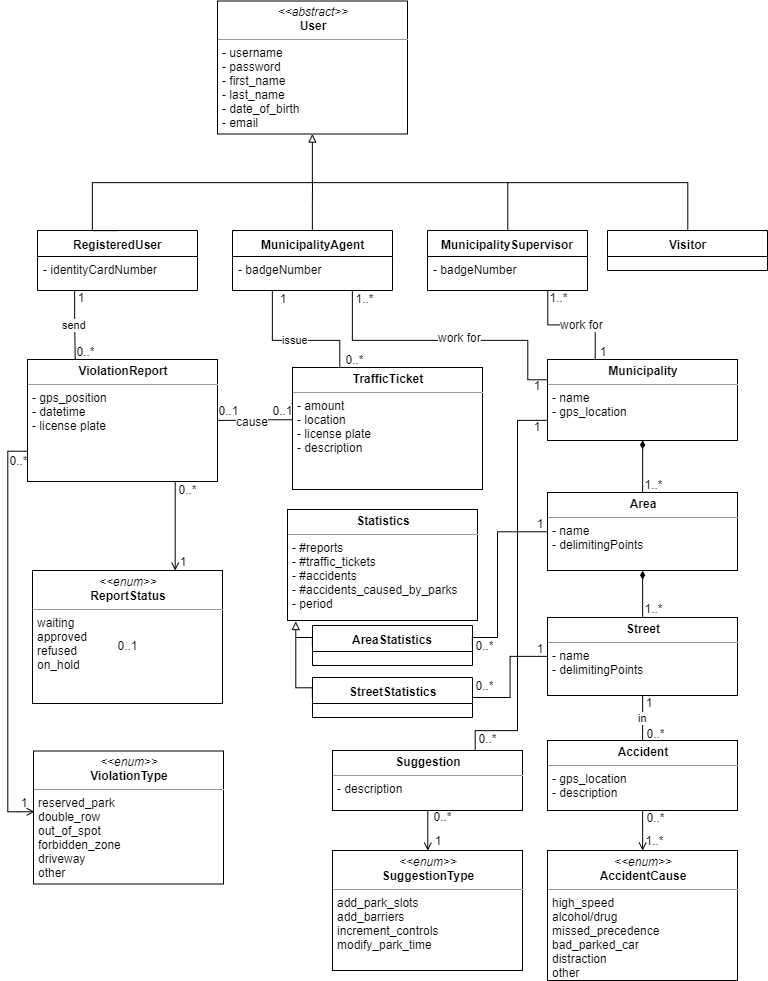
\includegraphics[width=\textwidth]{ClassDiagram}
\caption{UML Class Diagram}
\label{fig:class-diagram}
\end{figure}
Some data appear to be duplicated in the \textit{TrafficTicket} class but it needs to be considered the fact that the application will receive also data about traffic tickets which have not been issued as a consequence of a SafeStreet report, but instead have been independently issued by the local police in their traditional control activities. They are necessary to correctly build statistics and they need to include data which are already present in the corresponding report, when it exists.\\
For what concerns the \textit{Accidents} here it has been supposed a representation for all types of accidents, coming from the municipality data, then the system will be able to discriminate the ones related to parking violations.\\
In figure \ref{fig:state-diagram1} is reported an \textit{UML State Diagram} to clearly represent the state evolution of a \textit{ViolationReport}, which is the main object which change its state in the time, while the other ones do not present significant evolutions from this point of view.
\begin{figure}[hp]
\centering
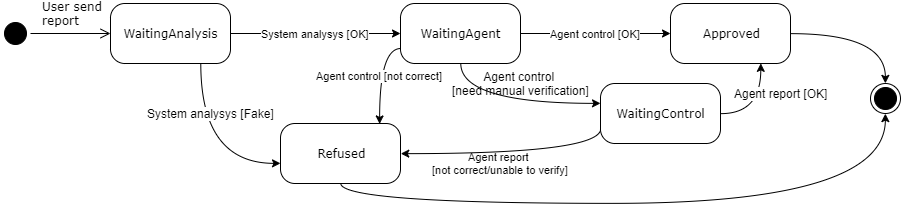
\includegraphics[angle=90, scale=0.6]{StateReport}
\caption{UML State Diagram for ViolationReport}
\label{fig:state-diagram1}
\end{figure}
\section{Product functions}

In this part are underlined the main functions offered by SafeStreets, divided by the users that can actually have access to them.

\subsection{Visitor}

\subsubsection{Registering to the application}

The system offers the possibility to Visitors to register and actually become users of the application. When registering the visitor needs to provide his name, surname, birthdate, fiscal code and identity card number. They are mandatory so if some of them is not provided then the registration process fails.
 
\subsection{User}

\subsubsection{Reporting a violation}
This is the most important function offered by SafeStreets. This function allows Users, when logged in, to report a potential violation that has occured in the streets. 
They can achieve that by inserting some mandatory data. When reporting a violation, a user must insert the type of violation that has been detected ( missing park disk, car illegally parked in the bike lane, car illegally parked in some reserved parking spot, not paid parking disk).
Subsequently, the user must provide at least one picture of the violation. Through the pictures, the user should provide clear evidence of the violation and the vehicle involved (in particular the license plate) before sending the report for a verification to the server. Optionally, the user can help recognition providing the license plate of the vehicle as plain text. Before sending the report, the application attaches to it the current position of the User (using GPS position), date and time of the report (taken through the network).

\subsection{Municipality agent}
\subsubsection{Authority agent registering}
Differently from the function previously explained and meant for normal Users, this function is only meant for Municipality agents. Each agent can register to SafeStreet to exploit his services as agent. He needs to provide his name, surname, birthdate and rank. After providing a password, the registration is sent for a verification to the municipality service and completed if the data inserted is correct. An ID code is then given to the agent to be uniquely identified.

\subsubsection{Violation checking}

This function is provided if and only if the municipality involved has installed the service needed to exploit SafeStreet data. After logging in as a municipality agent, the system notifies the agent about all the current not resolved reported violations. The agent can visualize individually each report, starting from the older one in terms of date and time, checking if the report corresponds to an actual violation. He can either directly emit a traffic ticket or send an agent directly on the street to check and eventually emit the ticket. At the end he can file the report and check the next report on the queue, if present.
Additionally, when logged in, the agent is notified of new incoming reports. 

\subsection{Municipality supervisor}

\subsubsection{Suggesting possible solutions} 
This function consists of a task periodically executed by the system (e.g. once a month) which tries to analyze reported violations, issued tickets, accidents information and data about the streets network coming from the municipality to suggest possible interventions to increase the safety (e.g. add barriers, create new park spots, increase the allowed parking time, send more agents in a certain area in certain hours...). When the system finds new suggestions it sends them to the municipality supervisors.

\subsubsection{Getting sensible information}
This function allows logged in municipality supervisors to retrieve information about the vehicles with the highest number of violations in a selected area. The system must return information belonging to the supervisor's area of competence, communicated during the registration process.

\subsection{Everyone} 

\subsubsection{Consulting statistics}
This function allows visitors, users, municipality agents or supervisors to retrieve information about the streets and areas with the highest frequency of violations; it is possible to retrieve statistics and trends about the accidents correlated to the parking violations, the effectiveness of SafeStreet initiatives and the issuing of traffic tickets. The information provided must be mined by the system from the reported violations, crossed with information from municipality. The system must not allow user to see confidential data about other people; it must allow the user to choose a topic: areas with most accidents, areas with the highest number of traffic tickets issued or areas where there have been the best improvements and in the end the system must show to the user the information about the topic selected.



\section{User characteristics}
The users of the service are the following:
\begin{itemize}
\item \textit{Visitor}: a non-logged user which can only consult statistics about areas with the highest frequency of violations, highest rate of accidents related to the violations, traffic tickets issued and safety improvements. 
\item \textit{User}: an identified user which, in addition to the \textit{visitor}, can report a parking violation, sending the details to the municipality authorities.
\item \textit{Municipality agent}: an agent of the local police which is notified about the violation reports for his municipality and can decide whether to immediately send a traffic ticket to the person responsible for a certain violation or to send an agent on the place to verify it and possibly discard it.
\item \textit{Municipality supervisor}: he has a full access to the application data, including all statistics and the suggestions to improve safety in the most dangerous areas.
\end{itemize}
\section{Assumptions, dependencies and constraints}
\subsection{Dependencies and constraints}
\label{SS-Dep&Const} 
The presence of some services provided by the municipalities is necessary to make all SafeStreet functions operative. In particular the following services are requested:
\begin{itemize}
\item \textit{Identity Card Check}: allows to retrieve data of a person given its identity card number.  It's request for a strong user authentication.
\item \textit{Accidents Information}: return information about the accidents occurred in the municipality streets, with position and causes.
\item \textit{Traffic Ticket Issue}: allows to send traffic tickets to a certain person by a certain agent
\item \textit{Agents Identity Check}: allows to check the identity of a registering agents given his personal data, including his badge number. 
\end{itemize}
\subsection{Domain Assumptions}
Here are shown the domain assumptions:
\begin{itemize}
\item{[D1]}GPS is always precise, giving the position with an error of maximum 5 meters.
\item{[D2]}Smartphone cameras have enough resolution to enable recognizing algorithms
\item{[D3]}Reported violation are always checked by an agent 
\item{[D4]}The identity card is unique for each person.
\item{[D5]}Each person has only one identity card.
\item{[D6]}The municipalities always issue traffic tickets if the reported violation is real and either pictures are clear or the agent on the street witnesses it directly.
\item{[D7]}Every registered municipality agent is associated with a unique ID.
\item{[D8]}Every municipality that uses Safestreet has at least 1 Agent and 1 supervisor that are in charge for managing SafeStreet services.
\item{[D9]}Every agent and supervisor works for exactly one municipality.
\end{itemize}

\chapter{Specific Requirements}
\lipsum[1]
\section{Scenarios identification} 
Here are presented possible scenarios for different users.\\ \\

\textbf{Scenario 1. Report of a violation}\\
\\
Mark is a man in his thirties. He’s an employee at Esselunga supermarkets. One day, walking down the main street of his city he finds a car parked illegally in the middle of the bike lane. Mark is registered in the application SafeStreet. He takes out his smartphone and opens the application. After writing his credentials and logging in, he clicks the button “Report a violation” in the home page. He inserts the type of violation, so in this case he just writes “car illegally parked in bike lane”, and takes three different pictures of the car: one of the front of the car, clearly showing the license plate; the second showing the entire car and, in the background, the signal of bike lane; the third one highlighting important elements of the streets where the potential violation occurred, to help the matching of the photo with the GPS position of the user. He then confirms clicking on the “Confirm” button. The potential violation is now sent to the server for a verification. Finally, he closes the application and continues his walk.
\\
\\ 
\textbf{Scenario 2. The agent receives a notification and issues a traffic ticket}\\
\\
Lukas is a municipality agent that is working as usual at his desk and has the SafeStreet Web app opened in the background on his PC. While checking his papers he receives a notification from the SafeStreet. He opens the window of the app and finds that a new report has been made about a violation. Lukas clicks on the row linked to the new violation. He observes that the violation has been reported by a certain Gianluca Verdi. The pictures of the report clearly show the vehicle that has made the violation (not paid parking meter), his license plate and the place where the violation occurred. There is now enough evidence that allows Lukas to issue a traffic ticket to the owner of the vehicle.
\\
\\
\textbf{Scenario 2b. A policeman receives a notification and send an agent to control because the picture is not clear}\\
\\
Laura is a municipality agent that has just started her new day at work. She works in Milan’s police station. She starts her PC at her desk, opens Internet Browser and search for SafeStreet Web App. After logging in, the reported violation queue is filled with 10 notifications of new potential violations reported. She opens the first one and she discovers that the system wasn’t able to correctly identify the vehicle involved and the user hasn’t inserted the license plate as plain text to help recognition. She checks the pictures but she can’t find out what is written on the license plate. She tells his supervisor the problem, in order to send an agent to directly check in the place of the supposed violation (based on the GPS position sent by the user) and, possibly, to issue a traffic ticket.
\\
\\
\textbf{Scenario 3. A user checks for unsafe streets in his zone}\\
\\
Bob is a curious user that has the SafeStreet application installed in his iPhone 8 but is not registered in the SafeStreet database. One day, he witnesses an accident in the streets while driving his car, where a car hits a biker during a parking manoeuvre on a runs over a biker correctly biking in his bike lane.
As he goes home, he’s curious about the most dangerous and unsafe areas and streets in his city and he wants to see if the street where he saw the accident is one of them. He opens the SafeStreet application and clicks the button “Check statistics in a city”. After this, a new page opens in which Bob clicks on the “Check for most dangerous areas/streets”. The last click he does is on the “Search for a city using your GPS position” button. Now the screen shows a map with highlighted the most unsafe areas (with most accidents) in his city. Bob selects then the area in which he is interested in and he sees which are the most dangerous streets in the area. Bob discovers that the street he was searching for is the most dangerous one. Finally, Bob closes the application.
\\
\\
\textbf{Scenario 4. Needs to travel and searches for safe places for a car}\\
\\
Marie is a woman who often travels for work. She typically travels by car. She lives in Milan and this week she needs to go to Turin. He wants to know where she can safely park the car and take an hotel reservation. Before searching for an hotel, she takes out her Huawei and opens the SafeStreet application. She clicks the button “Check statistics in a city”. After this, a new page opens in which Bob clicks on the “Check for most dangerous areas/streets”. The last click he does is on the “Select a city you want” button. She chooses “Turin” among all the possible ones. Now she can use found information to look for safe zones near her workplace.
\\ 
\\
\textbf{Scenario 5. New intervention suggestion for an unsafe street}\\
\\
Marco is a local police supervisor in the municipality of Varese. He logins in the SafeStreet application and he sees a notification about a suggestion for an intervention to improve safety. He opens it and he reads that in Via Roma there have been a lot of reports and consequent tickets in the last months due to cars parked on the sidewalk. The system is suggesting to add barriers to prevent cars from going on the sidewalk. This seems a good suggestion for him, he will discuss it with the competent municipality sector. 
\\
\\
\textbf{Scenario 6. The user registers to the application}\\
\\
Luke and Walter are two close friends. Luke doesn’t know about SafeStreet application while Walter is a regular registered user of it. One day, Walter and Luke are walking down a road. Walter notices a potential violation and stops. He takes out his phone and opens the SafeStreet application. Luke asks Walter what he’s doing and Walter explains what SafeStreet is. Walter is pretty convincing and makes Luke install the application. Luke learns that to report violations he needs to register. So, he starts the process of registration providing his name, surname, birthdate, fiscal code and number of the identity card. After this, he creates his own unique username and the password. On screen, Luke sees that the registration has been successful. 
\\
\\
\textbf{Scenario 7. A supervisor wants to check see what areas are registering improvements since the municipality has started to use SafeStreet}\\
\\
Giulio is a local police supervisor in the municipality of Milan. It’s six months since they have started to use the SafeStreet application to receive report from citizens about parking violations and he want to check what benefits it has brought. He opens the web application, he logins inserting his credentials and he clicks on Improvements under the Statistics section. Here he can see what streets have seen the best reduces in the number of issued tickets. He sees that a lot of central zones have seen reductions from 20 to 50%, while in the peripheral areas the numbers are much less substantial. He is happy because of this result, but he wants to improve it and he thinks to start a marketing campaign to encourage more people to use the application, especially in the peripherals. 
\\ 
\\
\textbf{Scenario 8. Marco wants to make a joke to a friend and send a fake report}\\
\\
Marco and Luigi are two very close friends. One day Marco decides it’s time to make a very not funny joke to his friend and he decides to use the SafeStreet application to make him receive a traffic ticket. He finds an illegally parked car, he photographs it and then he tries to modify the license plate in the photo with Luigi’s car license plate. He sends the report with the modified photo thinking about the face of Luigi when he will receive the ticket. 
Some weeks later he receives a letter from the judicial authority stating that they have started a criminal proceeding against him for the crime of slander (see [SLANDER]).
Probably he won’t do it another time. 
\\ 
\\
\textbf{Scenario 9. A municipality agent registers to the application}\\
\\
Ben is a new local police agent in the municipality of Bologna hired only two days ago and his supervisor says him that he has to register to the SafeStreet application. So Ben open the already installed application from his Computer and clicks on the "Register" button on the homepage. He inserts his name, surname, birthdate and rank, then he choooses his password, equal to "LKJVC89", and confirm the inputs. After the registration is processed, Ben receives his unique ID and is returned to the home page. He can now properly work.

\section{UML diagrams analysis}

\subsection{Use case diagram}

//insert Use case here

\subsection{Use case identification}
This part consists in all possible use cases taken from use case diagram and the scenarios previously described.\\ \\
\textbf{1. User logs in}
\\
\\
Actors: User
Entry condition: 
\begin{itemize}
\item The User needs to have the application opened
\end{itemize}
Flow of events:
\begin{itemize}
\item The User clicks on the login button
\item The user input his username (ID) and his password
\item The user clicks on the “confirm” button
\item The system redirects the taxi driver to his personal homepage
\end{itemize}
Exit conditions: 
\begin{itemize}
\item The user is successfully redirected to his personal homepage
\end{itemize}
Exceptions: 
\begin{itemize}
\item The code and password provided by the user are not correct. In this case, the system does not redirect the user to his personal homepage but notifies him that an error has been made and allows to input his code and password again
\end{itemize}
\textbf{2. User reports a violation} \\ \\
Actors: User\\
Entry condition:
\begin{itemize}
 \item The user must be logged in and on his personal homepage.
 \end{itemize}
Flow of events:
 \begin{itemize}
\item The user input clicks on the “Report violation” button.
\item The user sets the “type of violation” button to a desired value, chosen from a choice list.
\item The user clicks on the “take photos” button and complete the operation.
\item The user eventually fills the form “license plate”.
\item The user clicks on the “confirm” button and is redirected to his personal home page.
\end{itemize}
Exit conditions:
\begin{itemize}
\item The system checks the report and manages it, checking if images are corrupted and eventually forwarding the report to the municipality agent.
\item	Before confirming, the User clicks on the "Back” button and cancels the current report. Pictures are cancelled too. 
\end{itemize}
Exceptions: \\
There are no exceptions for this use case. 
\\
\\
\textbf{3. Agent or supervisor registers}
\\
\\
Actors: Municipality agent or Municipality supervisor \\
Entry condition:
\begin{itemize}
\item the agent or supervisor needs to have the Web App opened.
\end{itemize}
Flow of events:
\begin{itemize}
\item The agent/supervisor opens the application and arrives at the homepage.
\item The agent/supervisor clicks on the “Register” button.
\item The agent/supervisor input his name, surname, birthdate and rank.
\item The agent/supervisor input his choosen password.
\item	The agent/supervisorr clicks on the "Complete Registration" button.
\item The system processes the registration and send information to the Municipality Service.
\item The system notify the agent/supervisor about his new Unique Identifier (ID) and suggest to remember it.
\item The agent/supervisor clicks on the "Understood" button.
\item	The system redirects the agent/supervisor to login page.
\end{itemize}
Exit conditions:
\begin{itemize}
\item The agent/supervisor is successfully redirected to login page.
 \end{itemize}
Exceptions: 
 \begin{itemize}
 \item The name, surnamem birthdate and rank furnished by the agent are not found by the municipality service. In this case, the system does not redirect the agent/supervisor to the login page, but notifies him that an error has been made and allows to insert name, surname, birthdate, rank and password again.
\end{itemize}
\textbf{4. Agent or supervisor logs in }
\\
\\
Actors: Municipality agent or Municipality supervisor \\
Entry condition:
\begin{itemize}
\item the agent/supervisor needs to have the Web App opened.
\end{itemize}
Flow of events:
\begin{itemize}
\item The agent/supervisor opens the application and arrives at the homepage.
\item The agent/supervisor clicks on the “Login” button.
\item The agent/supervisor input his username and password.
\item	The agent/supervisor clicks on the log in button.
\item	The system redirects the agent/supervisor to his personal page.
\end{itemize}
Exit conditions:
\begin{itemize}
\item The agent/supervisor is successfully redirected to his personal page.
 \end{itemize}
Exceptions: 
 \begin{itemize}
 \item The username and password furnished by the agent/supervisor are not correct. In this case, the system does not redirect the agent/supervisor to his personal page, but notifies him that an error has been made and allows to input his username and password again.
\end{itemize}
\textbf{5. Checking statistics}
\\ \\
Entry condition: 
\begin{itemize}
\item The user needs to have the application opened
\end{itemize}
Flow of events:
\begin{itemize}
\item The user clicks on the Checking statistics button in the main page
\item The user chooses to get statistics either from his city or from another one
\item The user clicks on the statistics he wants to know 
\item After checking, user presses the Back button to return to the home page
\item The system asks the user if he wants to confirm with a “Yes” or “No” choice
\item The user presses the button he wants, confirming his choice
\end{itemize}
Exit conditions:
\begin{itemize}
\item User is successfully brought back to the home page
\end{itemize}
Exceptions: \\There are no exception in this case
\\ \\
\textbf{6. Supervisor checks potential intervention}
\\ \\
Actors: Supervisor
Entry condition: 
\begin{itemize}
\item The supervisor must be logged in. Possibly he have received a notification about a new available suggestion. 
\end{itemize}
Flow of events:
\begin{itemize}
\item The supervisor clicks on the “Recent Suggestions” button or clicks on the new suggestion notification.
\item The system redirects the supervisor to a page where he can choose between the ten most recent suggestions.
\item The supervisor chooses a suggestion.
\item The system shows the supervisor the whole text of the suggestion.
\item The supervisor clicks the “Done” button and is redirected again to his personal homepage.
\end{itemize}
Exit conditions:
\begin{itemize}
\item The supervisor is successfully brought back to his personal home page.
\end{itemize}
Exceptions:
\begin{itemize}
\item There are no recent suggestions, so the system notifies the supervisor about this exception. The system redirect the supervisor to his personal page.
\end{itemize}
\textbf{7. Agent checks a notified violation}
\\ \\
Actor: Municipality Agent \\ \\
Entry condition: 	
\begin{itemize}
\item The agent needs to be logged in the municipality Web App
\end{itemize}
Flow of events:
\begin{itemize} 
\item The agent receives the notification through the Web App of a new incoming report violation
%\item  If the reported violation queue is not empty, the agent clicks on another report.
%\item  If the reported violation queue is empty, the agent clicks on the small rectangle in the main page to see more about the new violation
\item Clicking on it, or entering in the Reports section, the system shows him the first report in the queue.
\item If the pictures are not clear enough, the agent contacts the supervisor to send an agent in the street to check and in the meanwhile he can put the report on hold by clicking on the button "On Hold".
\item If he is sure that what is reported is not a violation he can discard the report with the button "Discard". Before doing this he can possibly retrieve data about the author of the report, clicking on the button "Author".
\item Otherwise the agent clicks the "Send ticket" button to file the report and send a ticket to the recognized owner of the vehicle. The system allows him to specify the amount of the ticket and a description.
\end{itemize}
Exit conditions:
\begin{itemize}
\item The violation is filed and the agent can continue with the next report in the queue, if it is not empty.
\end{itemize}
Exceptions: 
\begin{itemize}
\item The municipality service used to issue traffic tickets is unreachable: in this case the system informs the agent and does not fill the report. The agent can retry until the system answers correctly.
\end{itemize}
\textbf{8. User registers to the Application}
\\ \\
Actor: Visitor \\ \\
Entry condition: 
\begin{itemize}
\item User needs to have the application opened in the main page
\end{itemize}
Flow of events:
\begin{itemize}
\item User clicks on the “sign in” button.
\item User provides the required information: fiscal code, identity card number, name username and birthdate;
\item User provides a Username and a password;
\item User clicks on “Confirm” button
\end{itemize}
Exit conditions: 
\begin{itemize}
\item The registration is completed and a message of confirmation is sent to the user, redirecting him to the main page of the application
\end{itemize} 
Exceptions: 
\begin{itemize}
\item The username provided is already in use the system shows an error message to the user; he has to insert a new Username (and password)
\item The sensitive information inserted are not correct (fiscal code or identity card number). The system shows an error message and the user has to insert again all his informations.
\item User doesn’t complete the registration process by pressing the “back” button in the page. He’s redirected to the main page.
\end{itemize}


\subsection{Sequence diagrams}
Here are reported some UML Sequence Diagrams for the most interesting use cases: \\
\begin{figure}[H]
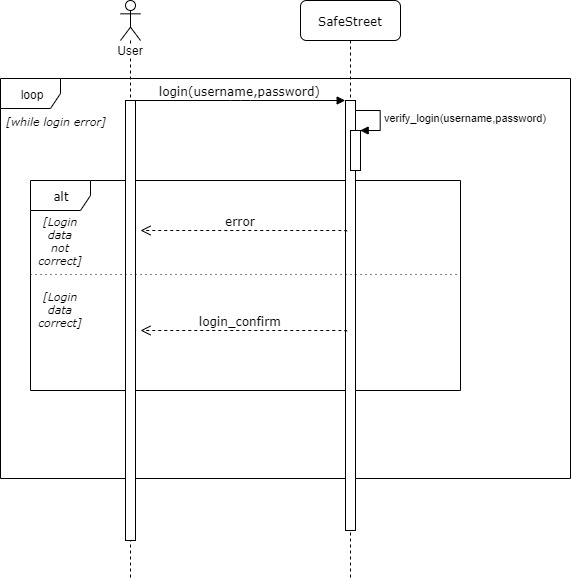
\includegraphics[width=\textwidth]{SequenceUserLogin}
\caption{Sequence diagram for use case n.1 (User logs in) }
\label{fig:seq-userlogin}
\end{figure}

\begin{figure}[H]
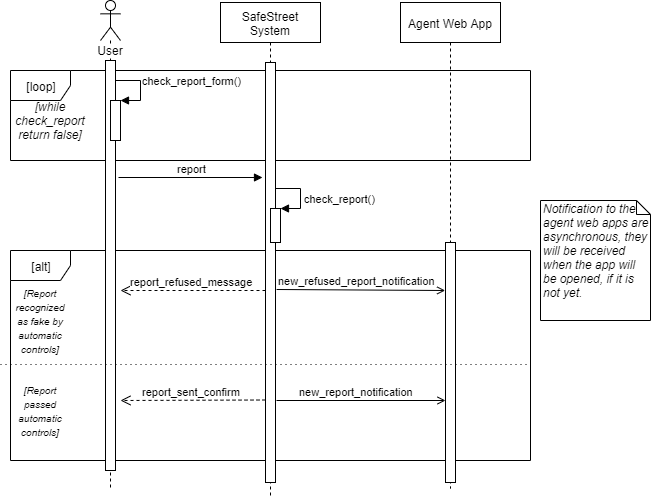
\includegraphics[width=\textwidth]{SequenceSendReport}
\caption{Sequence diagram for use case n.2 (User reports a violation) }
\label{fig:seq-userreport}
\end{figure}

\begin{figure}[H]
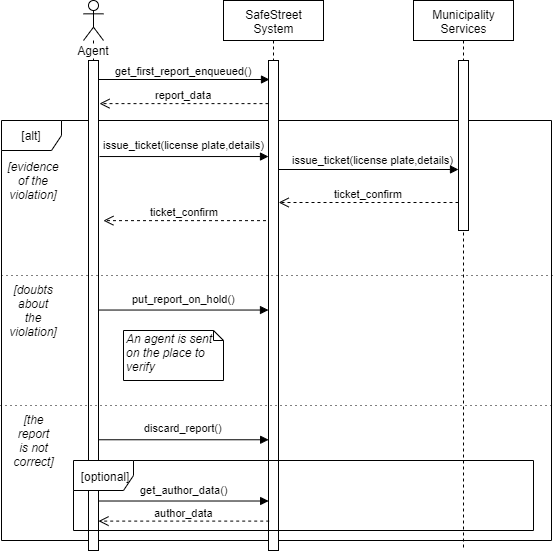
\includegraphics[width=\textwidth]{SequenceAgentCheckReport}
\caption{Sequence diagram for use case n.7 (Agents checks a notified violation) }
\label{fig:seq-agentcheckreport}
\end{figure}

\begin{figure}[H]
\centering
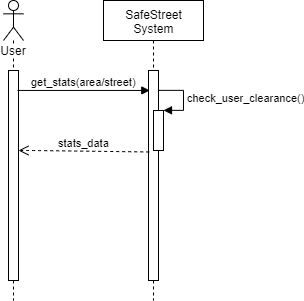
\includegraphics[scale=0.7]{SequenceCheckStatistics}
\caption{Sequence diagram for use case n.5 (Checking statistics) }
\label{fig:seq-checkstats}
\end{figure}



\section{External interface requirements}
\subsection{User Interfaces}
\lipsum[1]
\subsection{Hardware Interfaces}
No hardware interfaces are provided, being SafeStreet just a software system.
\subsection{Software Interfaces}
The system does not provide any software interface, because there are no other application which actually need to retrieve data from it. \\
The system has to call the municipalities services to retrieve some information (see \ref{SS-Dep&Const} ).
\subsection{Communication Interfaces}
The communication between users and SafeStreet servers exploit internal APIs through the \textit{HTTPS} protocol. The same is assumed for the communication with the municipalities systems. \\
For the \textit{users} the communication is unidirectional, in the sense that they cannot receive requests/notification by the server, all communications start from them. \\
The \textit{municipality agents} can be notified from the server when there are new report to be analyzed. \\
The \textit{municipality supervisors} can be notified about suggestions for interventions on the most unsafe areas.
\section{Functional requirements}
\lipsum[1]
\section{Performance requirements}
Performance requirements are not particularly critical for the system, but it is anyway desirable that all requests sent to the server are answered within 1 second, to assure a good user experience. \\
The server infrastructure will be designed to be scalable so that it will be possible to adapt it to the increment of users when the app diffusion will increase.
\section{Design constraints}
%\subsection{Standards compliance}
\subsection{Regulatory policies}
The application will only record the data strictly correlated to the reported violations and the data provided by the users during the registration. This data will be used only for the purposes of the system and will be treated confidentially, according to the \textit{GPDR} rules.\\
In particular the statistical analyses performed will never show publicly any information which can be related to a specific person.
\subsection{Hardware and software limitations}
The following requirements are necessary to install the mobile application:
\begin{itemize}
\item \textit{Operating system}: Android 5+ or iOS 9+
\item \textit{Hardware}: to allow the access as logged user the smartphone needs to have a camera and a GPS sensor
\end{itemize}
The camera is needed to take photos of the violations and the GPS is necessary to automatically record the position. The users have to give the relative permissions to the application. A base necessary requirement to use any functionality is the presence of an internet connection.\\
This requirements allow the majority of people to use the application \mbox{(see \hyperref[ref:os-stats]{\textit{[OS-STAT]}}).}\\
The authorities have the possibility to use a web interface, accessible through every modern browser.\\
Everyone can consult the publicly available statistics also through the \textit{SafeStreet website}, with any modern browser.
\subsection{Any other constraints}
//PROBABLY NOTHING
\section{Software system attributes}
\subsection{Reliability-Availability}
The availability is not a critical requirement, but the system has to guarantee a 99\% of uptime (max 3.65 days/year of downtime) to ensure that the users can normally use it.
\subsection{Security}
Security is a critical requirement for this system, considering the confidential information that are transmitted through it. It is assured by the use of the \textit{HTTPS} protocol for all communications and by the follow of the best security practices for the servers management, protecting them with IDS, maintaining the data ciphered and assuring the access only to the authorized users. \\
Every activity performed by municipality agents and supervisors will be logged to ensure its traceability.
\subsection{Maintainability}
The system will be realized following the best software engineering practices to ensure its maintainability and expandability in the future.
\subsection{Portability}
The system is actually designed to be compatible with most of Android and iOS devices (smartphones and tablets) and from the authorities side it can be accessed from any web browser, so it is very portable.
It will be important to maintain it compatible with the future releases of this two operating systems and with any other new operating system or device that will acquire an important market share.
\chapter{Formal Analysis using Alloy}
\lipsum[3]

\chapter{Effort spent}

\begin{center}
Nicola Rosetti \\
%\begin{tabular}{lll}
\begin{tabular}{p{2cm}p{1.5cm}p{7cm}}
\toprule
\textit{Date} & \textit{Hour} & \textit{Section} \\ \midrule
17-10-2019 & 1.5 h* & Goals \\
\bottomrule
\end{tabular}
\end{center}
\vspace*{1 cm}
\begin{center}
Simone Sartoni \\
\begin{tabular}{p{2cm}p{1.5cm}p{7cm}}
\toprule
\textit{Date} & \textit{Hour} & \textit{Section} \\ \midrule
17-10-2019 & 1.5 h* & Goals \\ \midrule
20-10-2019 & 4.5 h & Goals revision and requirements  \\ \midrule
22-10-2019 & 3 h & Goals and requirements revision \\ \midrule
23-10-2019 & 1.5 h & Use Case UML model design and draw \\ \midrule
24-10-2019 & 2 h & Goal and requirements revision, functions \\ \midrule
25-10-2019 & 2 h & Use Case UML model update \\ \midrule
27-10-2019 & 1.5 h & Use Cases writing \\ \midrule
29-10-2019 & 2 h & Use Case UML model and use cases revision \\ \midrule
31-10-2019 & 1 h & Scenario and use cases revision \\ 
\bottomrule
\end{tabular}
\end{center}
\vspace*{1 cm}
\begin{center}
Vittorio Torri \\
\begin{tabular}{p{2cm}p{1.5cm}p{7cm}}
\toprule
\textit{Date} & \textit{Hour} & \textit{Section} \\ \midrule
17-10-2019 & 1.5 h* & Goals \\ \midrule
20-10-2019 & 1 h & Users, Hardware and software limitations, goal refinement \\ \midrule
21-10-2019 & 1 h & Software, Hardware and Communication Interfaces, Performance requirements, Design constraints, Software system attributes \\ \midrule
22-10-2019 & 1 h & Goal and requirements revision \\ \midrule
23-10-2019 & 1 h & Goal and requirements revision \\ \midrule
26-10-2019 & 2 h & Scenarios, requirements, functions, scope \\  \midrule
28-10-2019 & 1.5 h & Product perspective and UML Class Diagram \\ \midrule
29-10-2019 & 1 h & State diagram and sequence diagram \\ \midrule
31-10-2019 & 0.5 h & Sequence diagram \\ \midrule
31-10-2019 & 1 h* & Alloy \\ \midrule
02-11-2019 & 1.5 h & Sequence diagrams \& minor fixes \\ \midrule
03-11-2019 & 4 h & Alloy \\ \midrule
04-11-2019 & 1 h & Alloy \\ 
\bottomrule
\end{tabular}
\end{center}
\textit{* Group work}

\chapter{References}
\begin{itemize}

\item \label{ref:os-stats} [OS-STAT] \href{https://gs.statcounter.com}{\textit{https://gs.statcounter.com}} - statistics on operating systems market share and versions diffusion

\item \label{ref:slander} [SLANDER] see art. 368, 370 and 69 c.p.p. (Italian law)

\end{itemize}

\end{document}
